There were a total of 3 shot days awared to this effort: WDMStopPow-16A, WDMStopPow-17A, and WDMStopPow-18A. Some details of all the shots are listed in Appendix \ref{apend:wdmData}. 

The objective of WDMStopPow-16A was to measure the stopping in WDM Be and (for the first time) Boron. This shot day featured Be plugs coated with Ag and Boron plugs coated with Vr. Both plugs used plastic layered gold cones with Zn foils attached for their x-ray Thomson Scattering shots. 

This shot day featured a few design flaws that unfortunately compromised the x-ray Thomson Scattering data. The first was the use of double-coned targets (shown in Figure \ref{fig:wdmDoubleCone}). The scattering from the second cone was thought to be problematic and was abandoned early on in the shot day. 

The second design flaw was the use of Zn foils that hung over the edge of the Au cone (See Figure \ref{fig:wdmOverhangFoil}). This overhanging cause direct emission from the Zn foil to hit the spectrometer and show up as an erroneously downshifted / upshifted x-ray line. This was overcome by only driving one of the two foils, to get useable data. This resulted in a measurement of the Be plasma's temperature at $6 \pm 5$ eV with an ionization of $Z < 2.2$. 

\begin{figure}[!h]
    \centering
    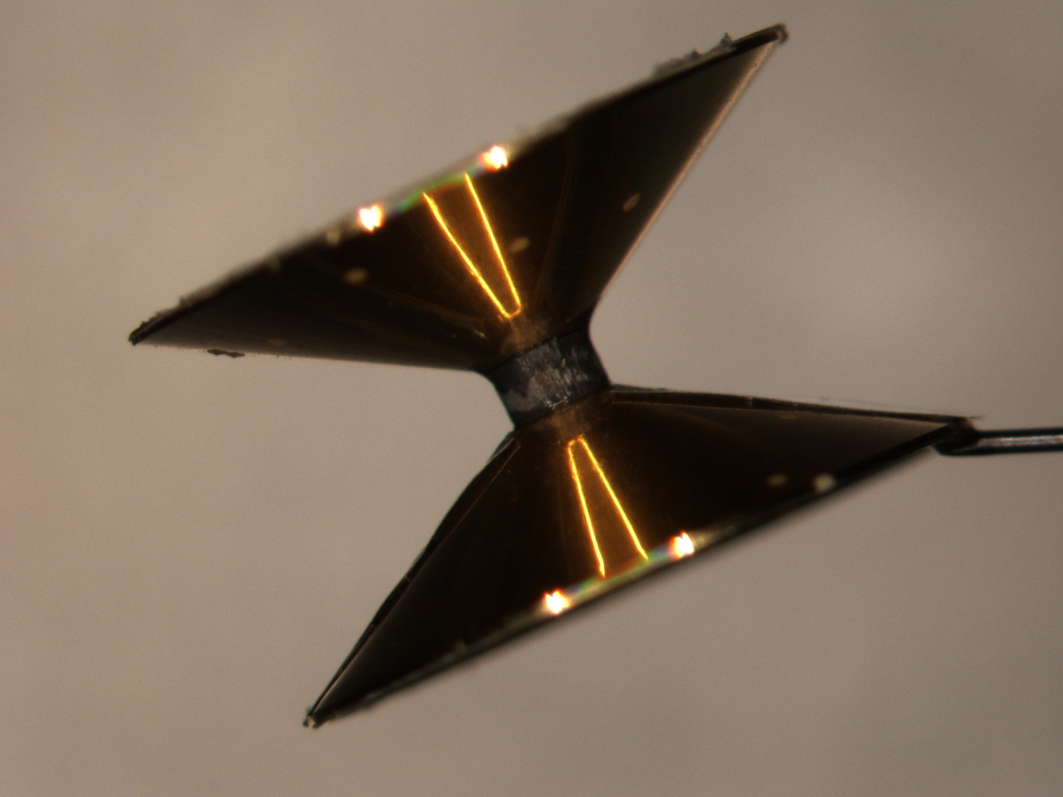
\includegraphics[scale=0.7]{Figures/wdmDoubleCone.pdf}
    \caption{Double cone X-ray Thomson Scattering Configuration}
    \label{fig:wdmDoubleCone}
\end{figure}

\begin{figure}[!h]
    \centering
    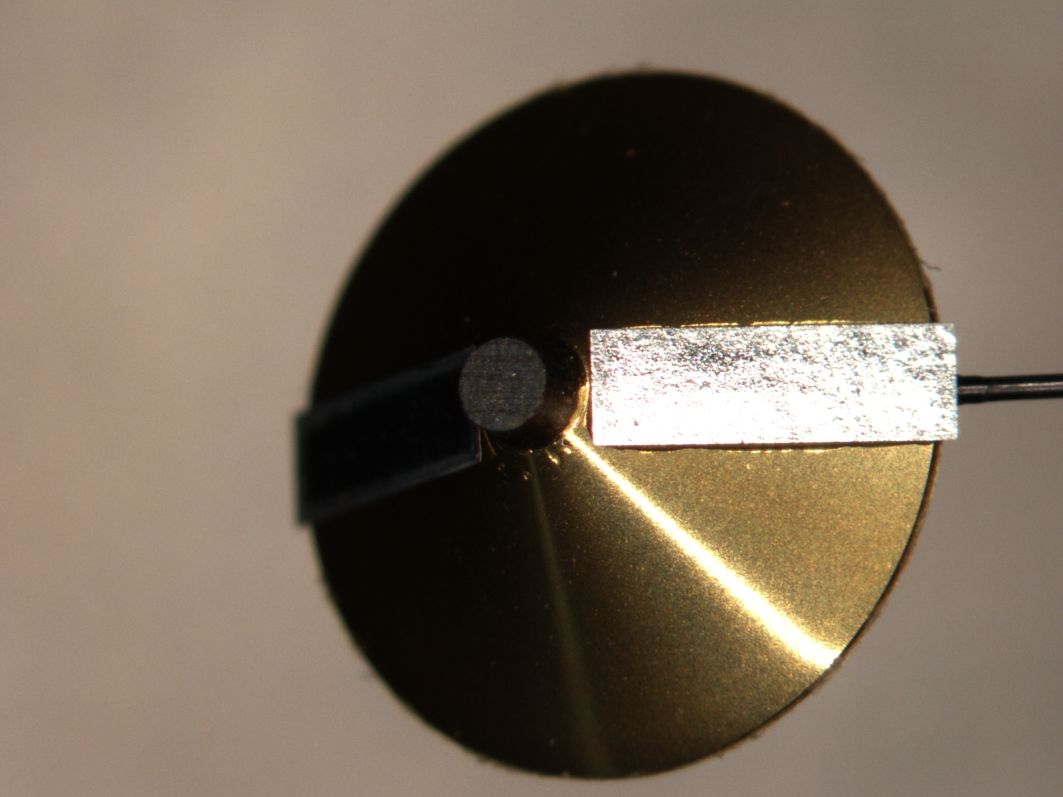
\includegraphics[scale=0.7]{Figures/wdmOverhangFoil.pdf}
    \caption[Overhanging Zn Foil Design Flaw]{Picture of a X-ray Thomson Scatter target with Zn foils overhanging the shield cone.}
    \label{fig:wdmOverhangFoil}
\end{figure}

The stopping power data from the shot day was mostly non-problematic, with a few unique features worth discussing. On shows where the target was driven to WDM, the WRF would measure both the source and downshifted spectra. While this shouldn't be possible given the nominal geometry parameters, it was a consistent effect on all shots. This is thought to be due to magnetic fields generated around the plug during the heating process. Another phenomenon that was observed was a reduction in the total number of protons. When compared to a spectra measured from any other line of sight, the downshifted spectra always saw less protons. This effect was exacerbated when the target was heated to WDM. This was thought to be due to some combination of scattering effects in the target and magnetic fields sweeping protons away from the detector. Example WRF data can be seen in Figure \ref{fig:exampleWarmWRFData}.

\begin{figure}[!h]
    \centering
    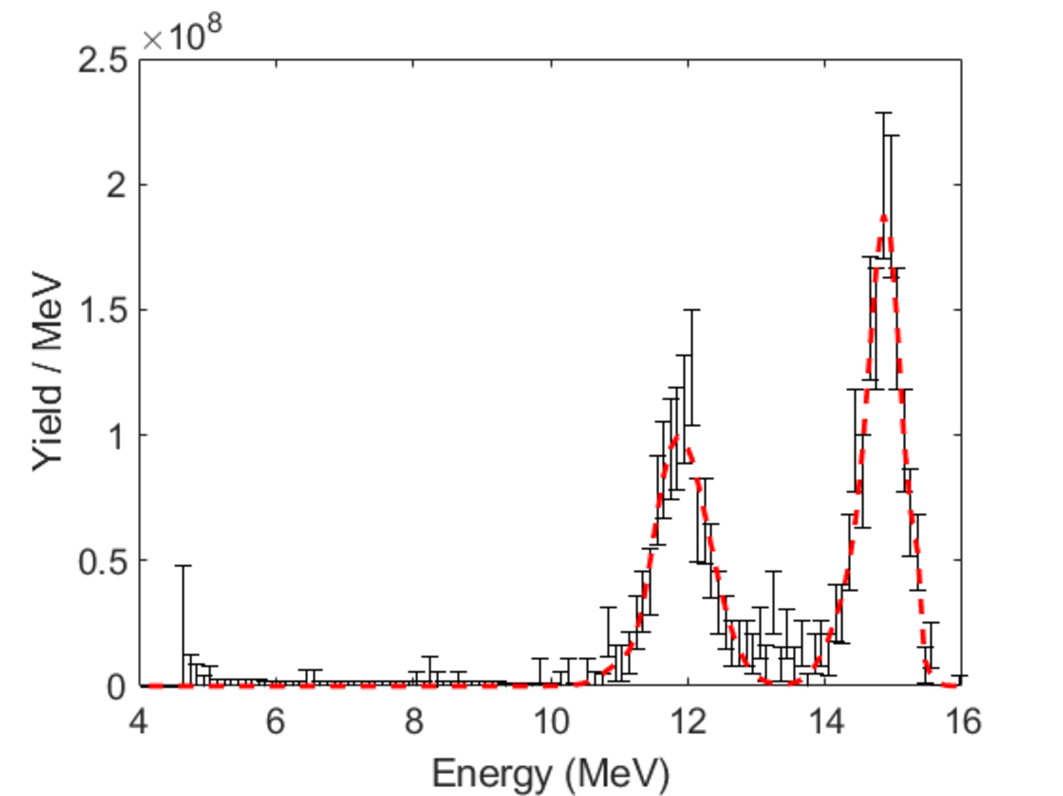
\includegraphics[scale=0.7]{Figures/wdmExampleWarmWRF.pdf}
    \caption[Example WRF Data from Om82291]{Example WRF Data from WDMStopPow-16A}
    \label{fig:exampleWarmWRFData}
\end{figure}

The objective of WDMStopPow-17A was to measure the stopping in WDM graphite and diamond. This shot featured both graphite and diamond plugs coated in Ni. Both plugs had a single Au cone with two Zn foils attached for their corresponding x-ray Thomson Scattering shots. 

This shot day achieved no usable x-ray Thomson scattering data sue to a design flaw with the heating material coating the plugs. The emission from Ni is very close to the emission from the scattered Zn spectra which ultimately corrupted the x-ray measurement. Additionally, Ni is an extremely good attenuator of the Zn x-rays which further reduced signal levels. Future shot days should avoid using any material with emissions in the vicinity of the scattered Zn spectra (8-9 keV).

The stopping power data also had issues. The counting statistics were poor due to the aforementioned yield reduction effects. With the carbon targets, these effects seem to have been exacerbated to the point of making the measurements unusable. Future experiments should consider thinner targets to compact scattering effects, and larger diameter targets to combat magnetic field effects.


The objective of WDMStopPow-18A was to measure the stopping in WDM Boron. This shot day featured the same Boron plug design from WDMStopPow-16A which used a Cr coating. Some Boron plugs used the familiar Au cone design, but others used a new 3D printed cone covered in Ta. 

This shot day was largely successful with great improvements being observed from the new Ta based shield cones. From the shot day, an electron temperature of $8.6^{+2.7}_{-3.1}$ eV and an ionization state of $Z < 3.1$ were observed using x-ray Thomson scattering. Additionally, the stopping power of an additional 2 cold targets and 4 warm targets was measured bringing the total up to 3 and 5 respectively. 

All of the stopping power data from Be targets is shown below in Figure \ref{fig:beWDMData}. When analyzing this data, there is no clear difference in the stopping between cold matter and WDM. This lack of difference is thought to be due to the low electron temperature and low ionization state inferred by the x-ray Thomson Scattering data. It is thought that the x-ray conversion efficiency of the Ag was lower than assumed. Future work should do a more thorough literature review of x-ray conversion drives to maximize this efficiency. 

\begin{figure}[!h]
    \centering
    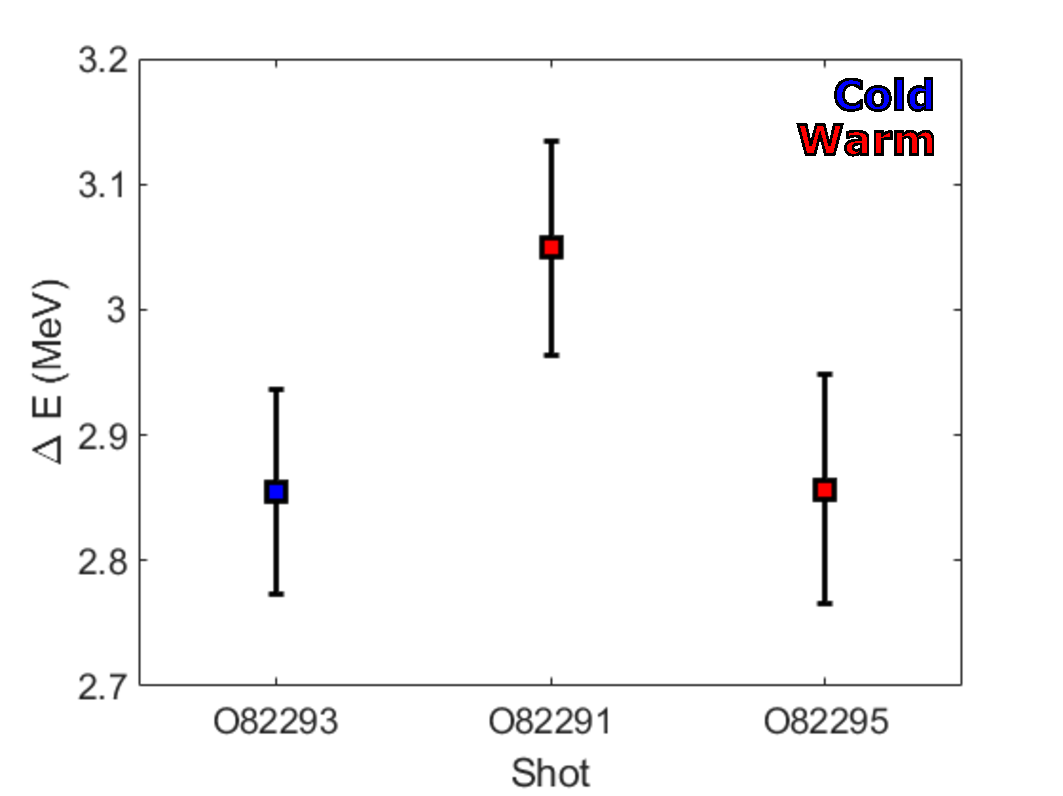
\includegraphics[scale=0.7]{Figures/beWDMData.pdf}
    \caption[Stopping power data from Be Targets]{All of the stopping power data from Be targets. There are a total of one cold shot (blue) and two WDM shots (red). The effective areal density seen by the protons was the same for each shot at $\rho L=101$ mg/cm$^2$.}
    \label{fig:beWDMData}
\end{figure}

All of the stopping power data from the Boron targets is shown below in Figure \ref{fig:boronWDMData}. There areal density of the boron targets varied from target to target due to manufacturing complications with working with boron. When plotted, there is a clear and consistent increase in stopping observed between WDM and cold. This is thought to be due to the increased electron temperature and ionization observed from the x-ray Thomson Scattering data.

\begin{figure}[!h]
    \centering
    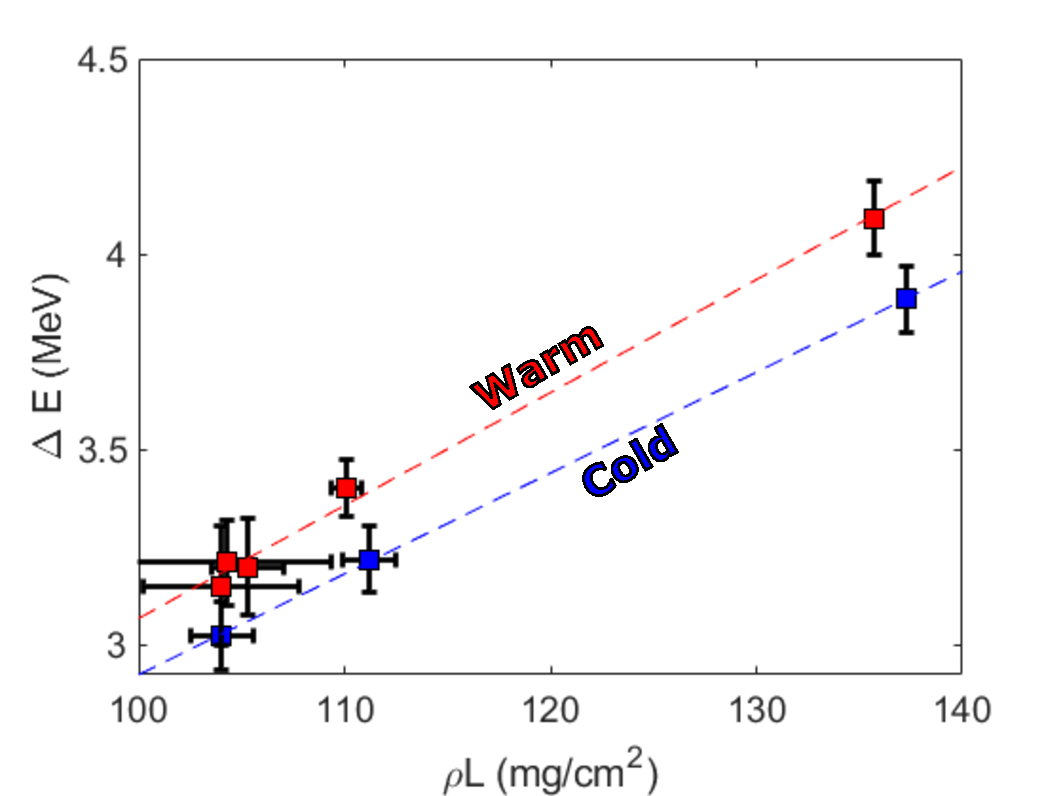
\includegraphics[scale=0.7]{Figures/bWDMData.pdf}
    \caption[Stopping power data from Boron Targets]{All of the stopping power data from Boron targets. There were a total of three cold shots (blue) and five WDM shots (red). The areal density of each target varied due to manufacturing differences.}
    \label{fig:boronWDMData}
\end{figure}

